\Chapter{MÉTHODOLOGIE}\label{sec:Methodologie}


La section méthodologique sera divisée en trois sections. La première présentera les jeux de données disponibles dans le contexte de la ville de Québec. La deuxième présentera une plan d'ensemble de la méthodologie et des moyens encourus pour faire l'inventaire du stationnement et la troisième.


\section{Données}
Le tableau \ref{tab:donnees_disponibles_Québec} résume les données disponibles pour la ville de Québec et leur source.
\begin{landscape}
\begin{table}[h!]
  \centering
   \begin{tabular}{l l p{.3 \linewidth} p{.15\linewidth} l } 
   \hline
   Géobase & Type & Description  & Source & Date public.\\ 
   \hline
   vdq-panneauxstationnement    & Points        & Panneaux de stationnement sur rue          & Ville de Québec / Données Québec  & 5 mai 2024 \\
   \hline
   vdq-bornesfontaines          & Points        & Bornes fontaines sur rue                   & Ville de Québec / Données Québec & 12 mai 2024 \\
   \hline
   vq\_reseau\_routier\_2023 & Polylignes    & Bords de voiries pour circulation automobile  & Ville de Québec / Geo-index  & 12 juin 2023\\ 
   \hline
   vq\_stationnement\_2021  & Polylignes    & Bords des aires de stationnement           & Ville de Québec / Geo-index & 8 mai 2021\\
   \hline
   vdq\_voie\_publique            & Lignes        & Centres de chaussées trottoirs séparés et pistes cyclables & Ville de Québec / Geo-index & 16 avril 2024 \\
   \hline
   Usages prédominants 2023  & Polygones & Usages prédominants du sol &   Ministère des Affaires municipales et de l'Habitation & 21 mai 2024 \\
   \hline
   Année de construction des chaussées & Polylignes & Année de construction des rues & Ville de Québec / Géoindex & 28 mai 2024 \\
   \hline
   highway & Polylignes & Centres de chaussées & \ac{OSM} & 13 mai 2024\\
   \hline
   parking & points et polygones & Stationnement recensés dans \ac{OSM} & \ac{OSM} & 2 mai 2024 \\
   \hline
    parking entrance & Points & Entrées de stationnement sous-terrains  & \ac{OSM} & 2 mai 2024 \\
    \hline
   \end{tabular}
   \caption{Géobases pour le territoire de la ville de Québec}
   \label{tab:donnees_disponibles_Québec}
\end{table}

\begin{table}[h!]
  \centering
   \begin{tabular}{p{0.18\linewidth} | p{0.1\linewidth} | p{0.3\linewidth} | p{0.3\linewidth}} 
   \hline
   Nom du champs & Type Contenu & Description  & Exemple\\ 
   \hline
   ID             & Entier    & Entier identifiant unique pour chaque panneau  & 370758 \\ 
   & & & \\
   TYPE\_CODE      & Texte     & Code d'identification de chaque type de panneau de stationnement & PP1016\\
   & & & \\
   DESCRIPTION     & Texte     & Texte imprimé sur le panneau & Stat. int. 16h-18h LUN À VEN (fl. dou.)\\
   \hline
   \end{tabular}
   \caption{Champs de la géobase de panneaux de stationnement de la ville de Québec \parencite{VilledeQuebec:PanneauxSignalisation:2024}}
   \label{tab:champs_geobase_stationnement_quebec}
\end{table}
\end{landscape}

\section{Illustration des données acquises}
La section suivante va donner un aperçu de quelques intersections typiques pour illustrer les données disponibles. Les mêmes quelque cas seront illustrés à des fins illustratives. Le but principal est d'illustrer les enjeux
\subsection{Illustration - Cas 1: Coin Gomin / Marguerite-Bourgeoys / Laurier}
Les figures \ref{fig:donnes_panneaux_Laurier} et \ref{fig:donnes_polygone_panneaux_Laurier} donnent un aperçu des données disponibles pour l'intersection nommée ci-dessus.
\begin{figure}[ht]
  \centering
  \begin{subfigure}{\linewidth}
    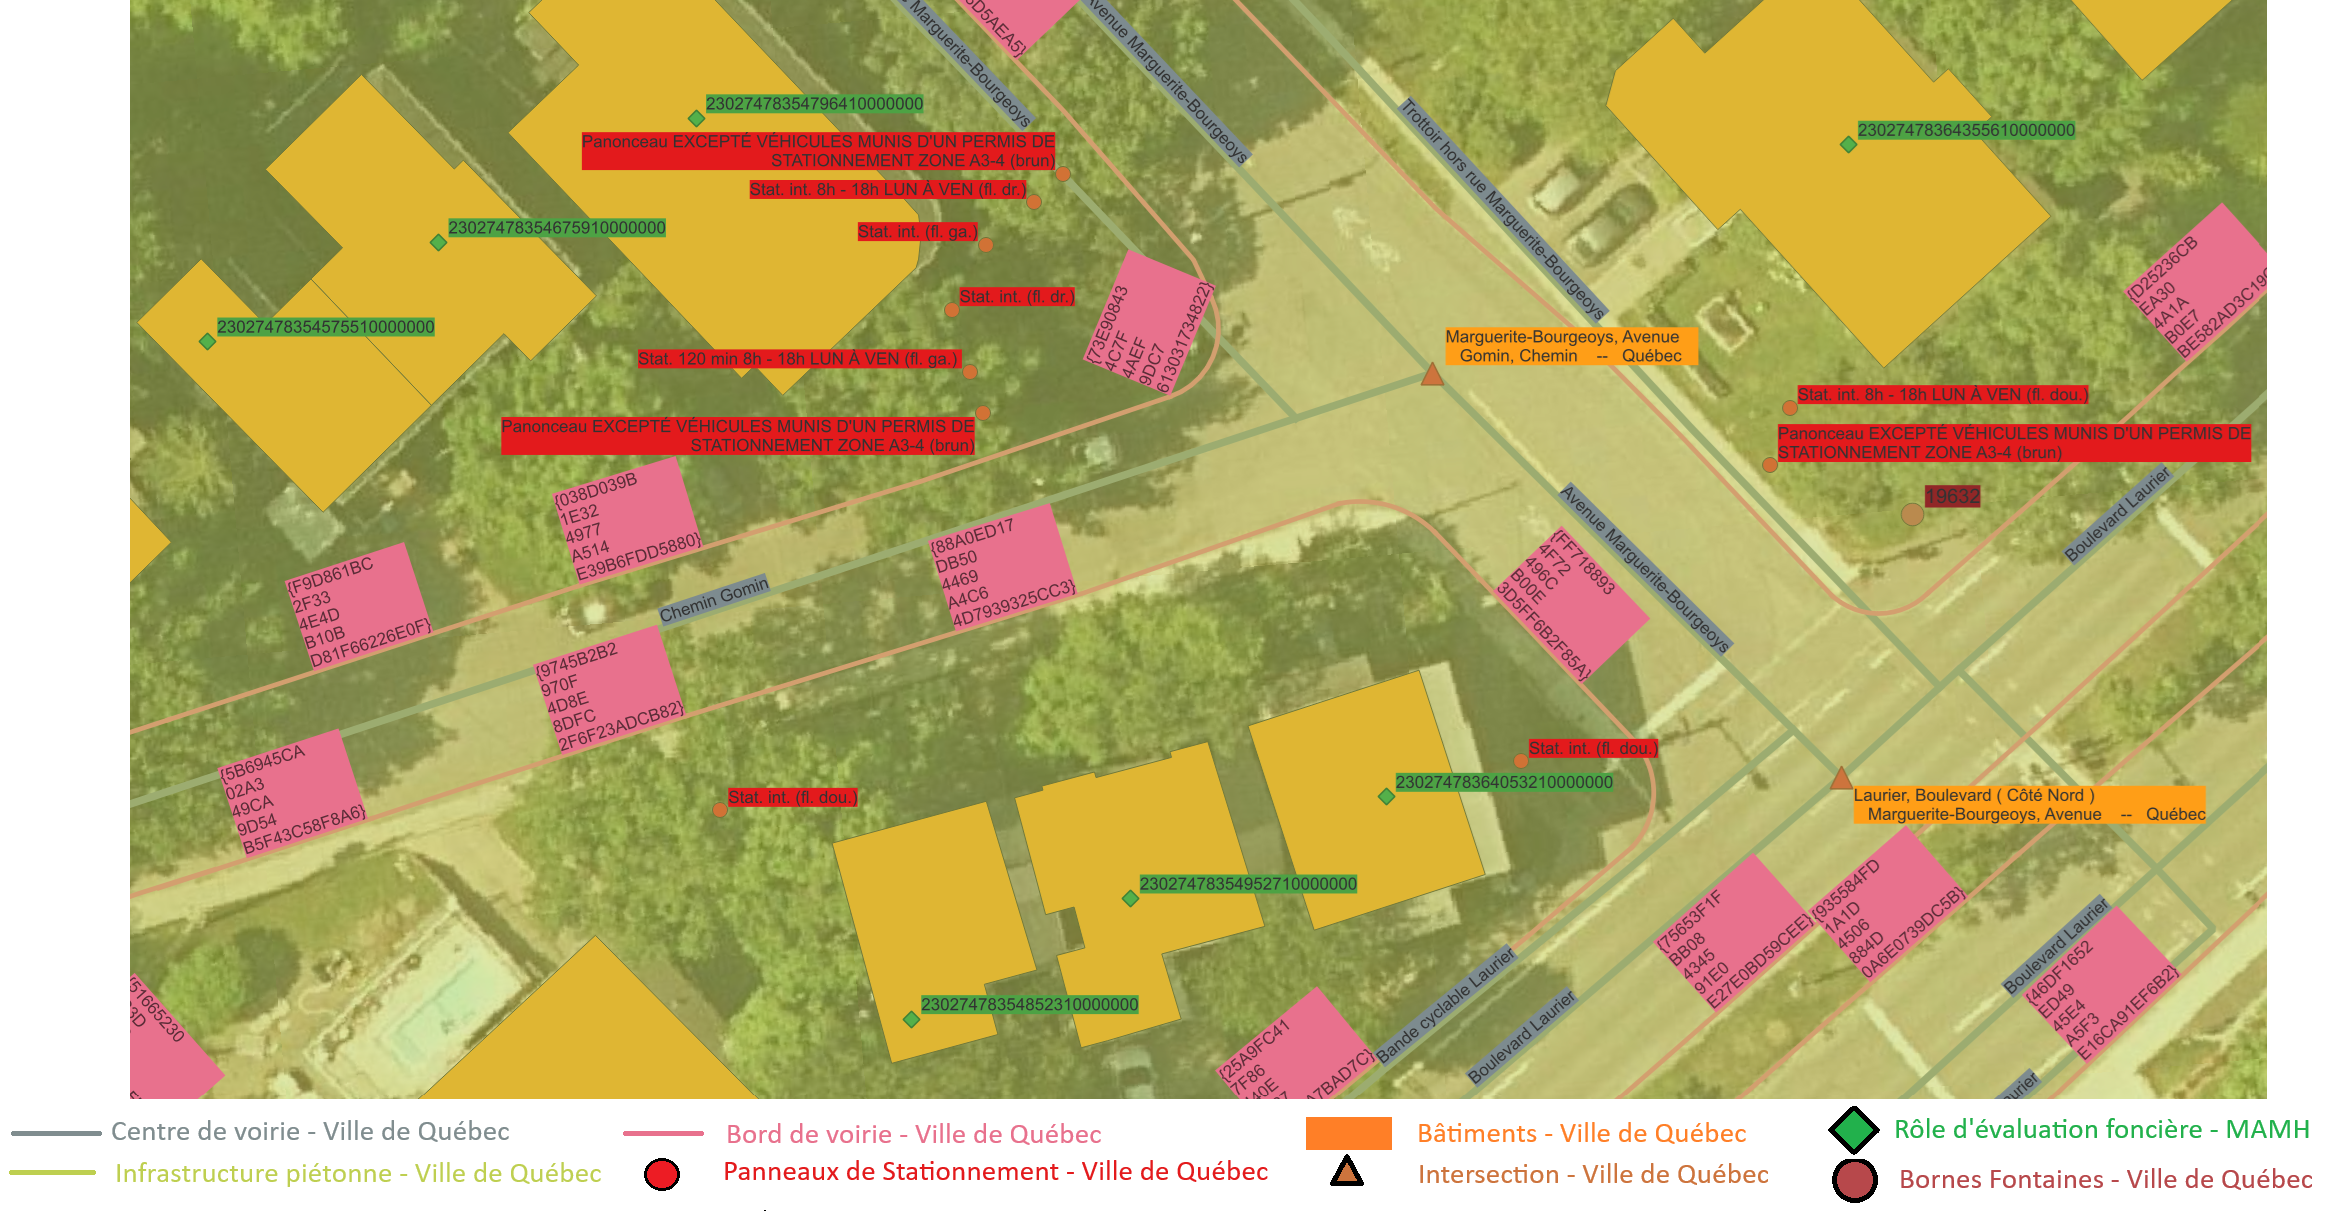
\includegraphics[width=1.0\textwidth]{images/donnees_disponible_Laurier_legende.png}
  \caption{Données linéaires pour l'inventaire de stationnement}
  \label{fig:donnes_panneaux_Laurier}
  \end{subfigure} \\
  \begin{subfigure}{\linewidth}
    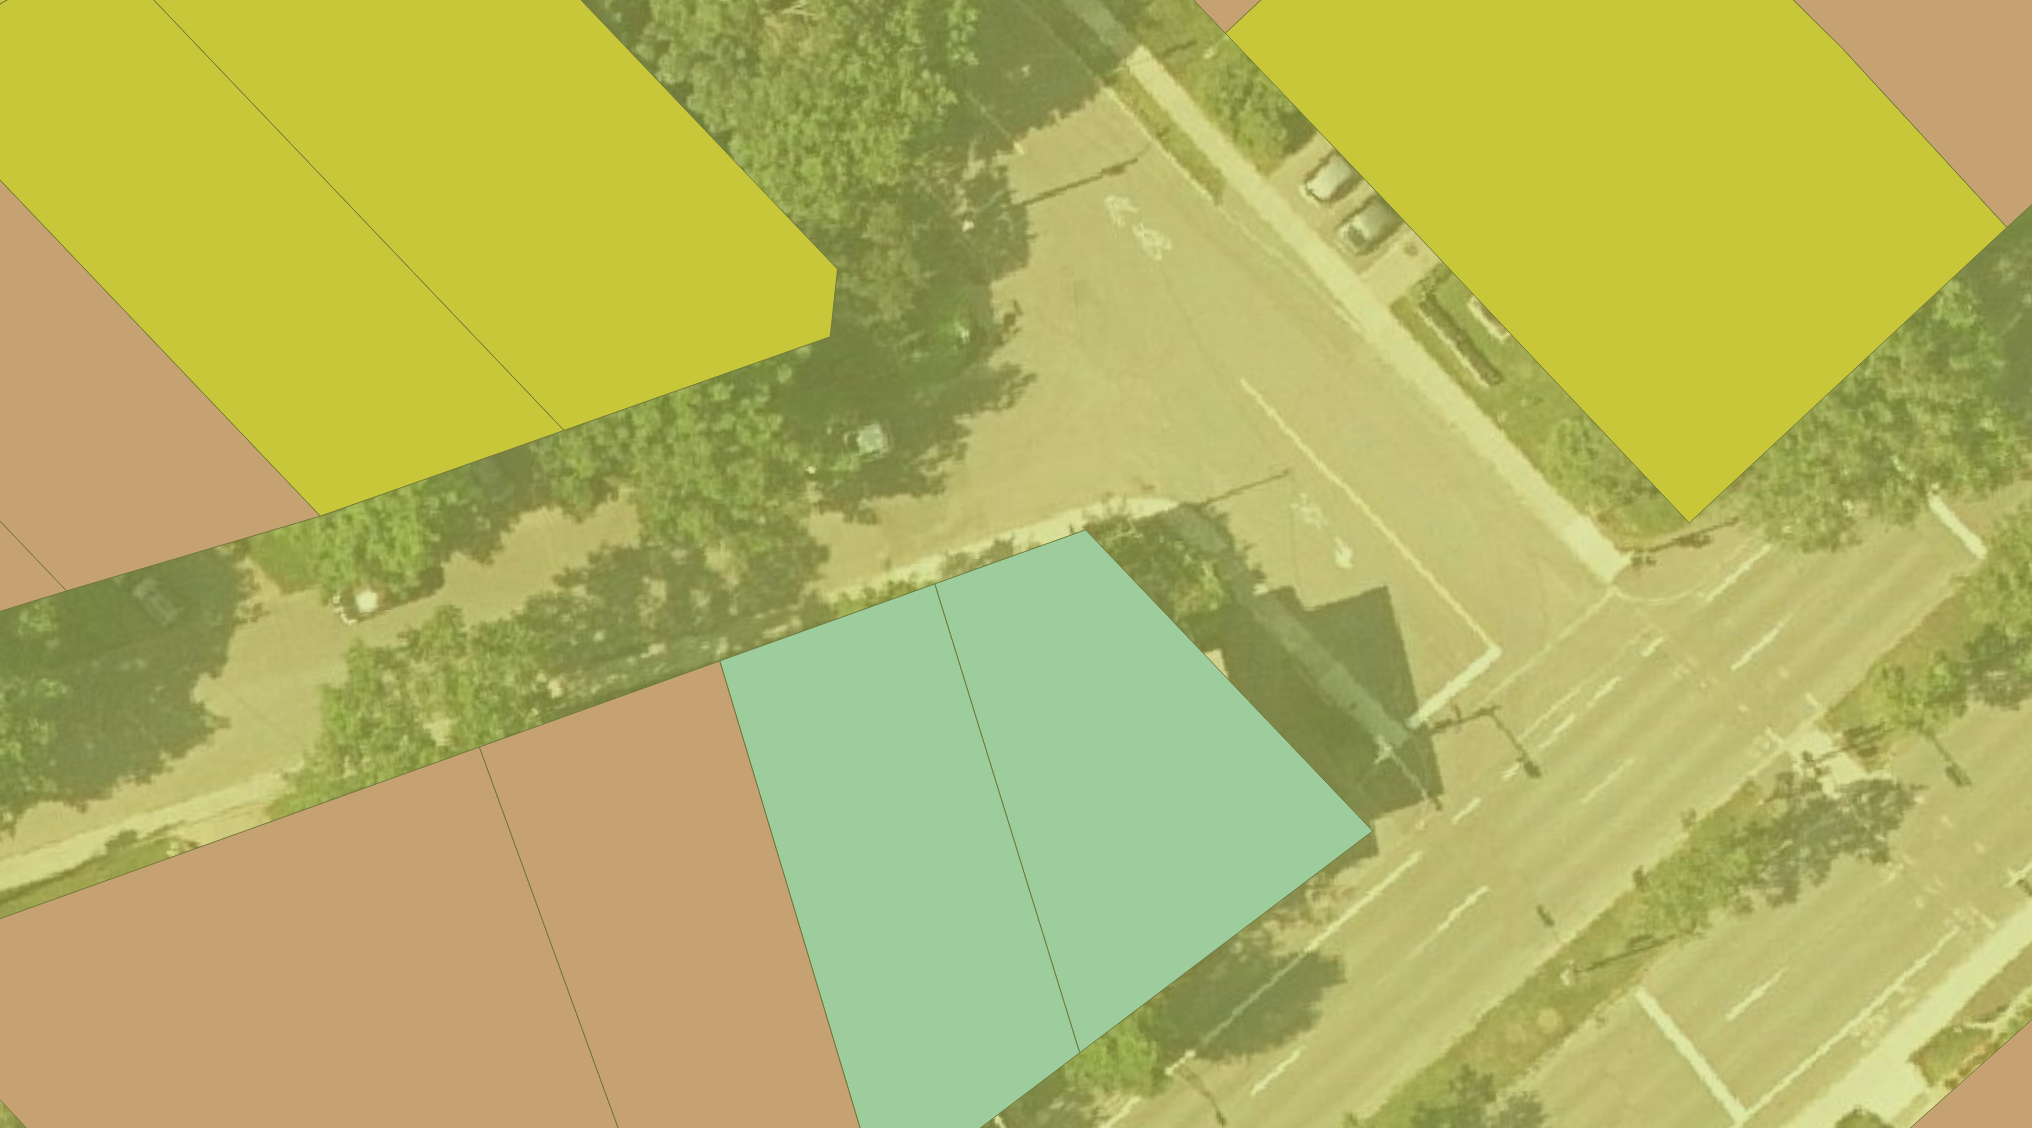
\includegraphics[width=1.0\textwidth]{images/utilisation_sols_Laurier.png}
  \caption{Données polygonales pour l'inventaire de stationnement}
  \label{fig:donnes_polygone_panneaux_Laurier}
  \end{subfigure}
  \caption{Données disponicles intersection Laurier}
\end{figure}

\FloatBarrier
\section{Données de panneaux de stationnement}
Des données de panneaux de stationnement sont disponibles en ligne sur le site de données ouvertes du gouvernement du Québec en lien avec la ville de Québec. Les champs associés aux données sont listés au Tableau \ref{tab:champs_geobase_stationnement_quebec}



Quelques distinctions de la base de donnée montréalaise sont aussi visibles dans la manière dont plusieurs panneaux à un même endroit sont traités. 

Dans le contexte de la ville de Québec, plusieurs panneaux sur un même poteau ne sont pas représentés au même endroit dans la base de données. La figure suivante donne un exemple à l'intersection de la rue Marguerite-Bourgeoys, du chemin Gomin et du Boulevard Laurier. On constate que les panneaux sur un même poteau sont localisés à des endroits différents

\begin{figure}[ht]
    \centering
    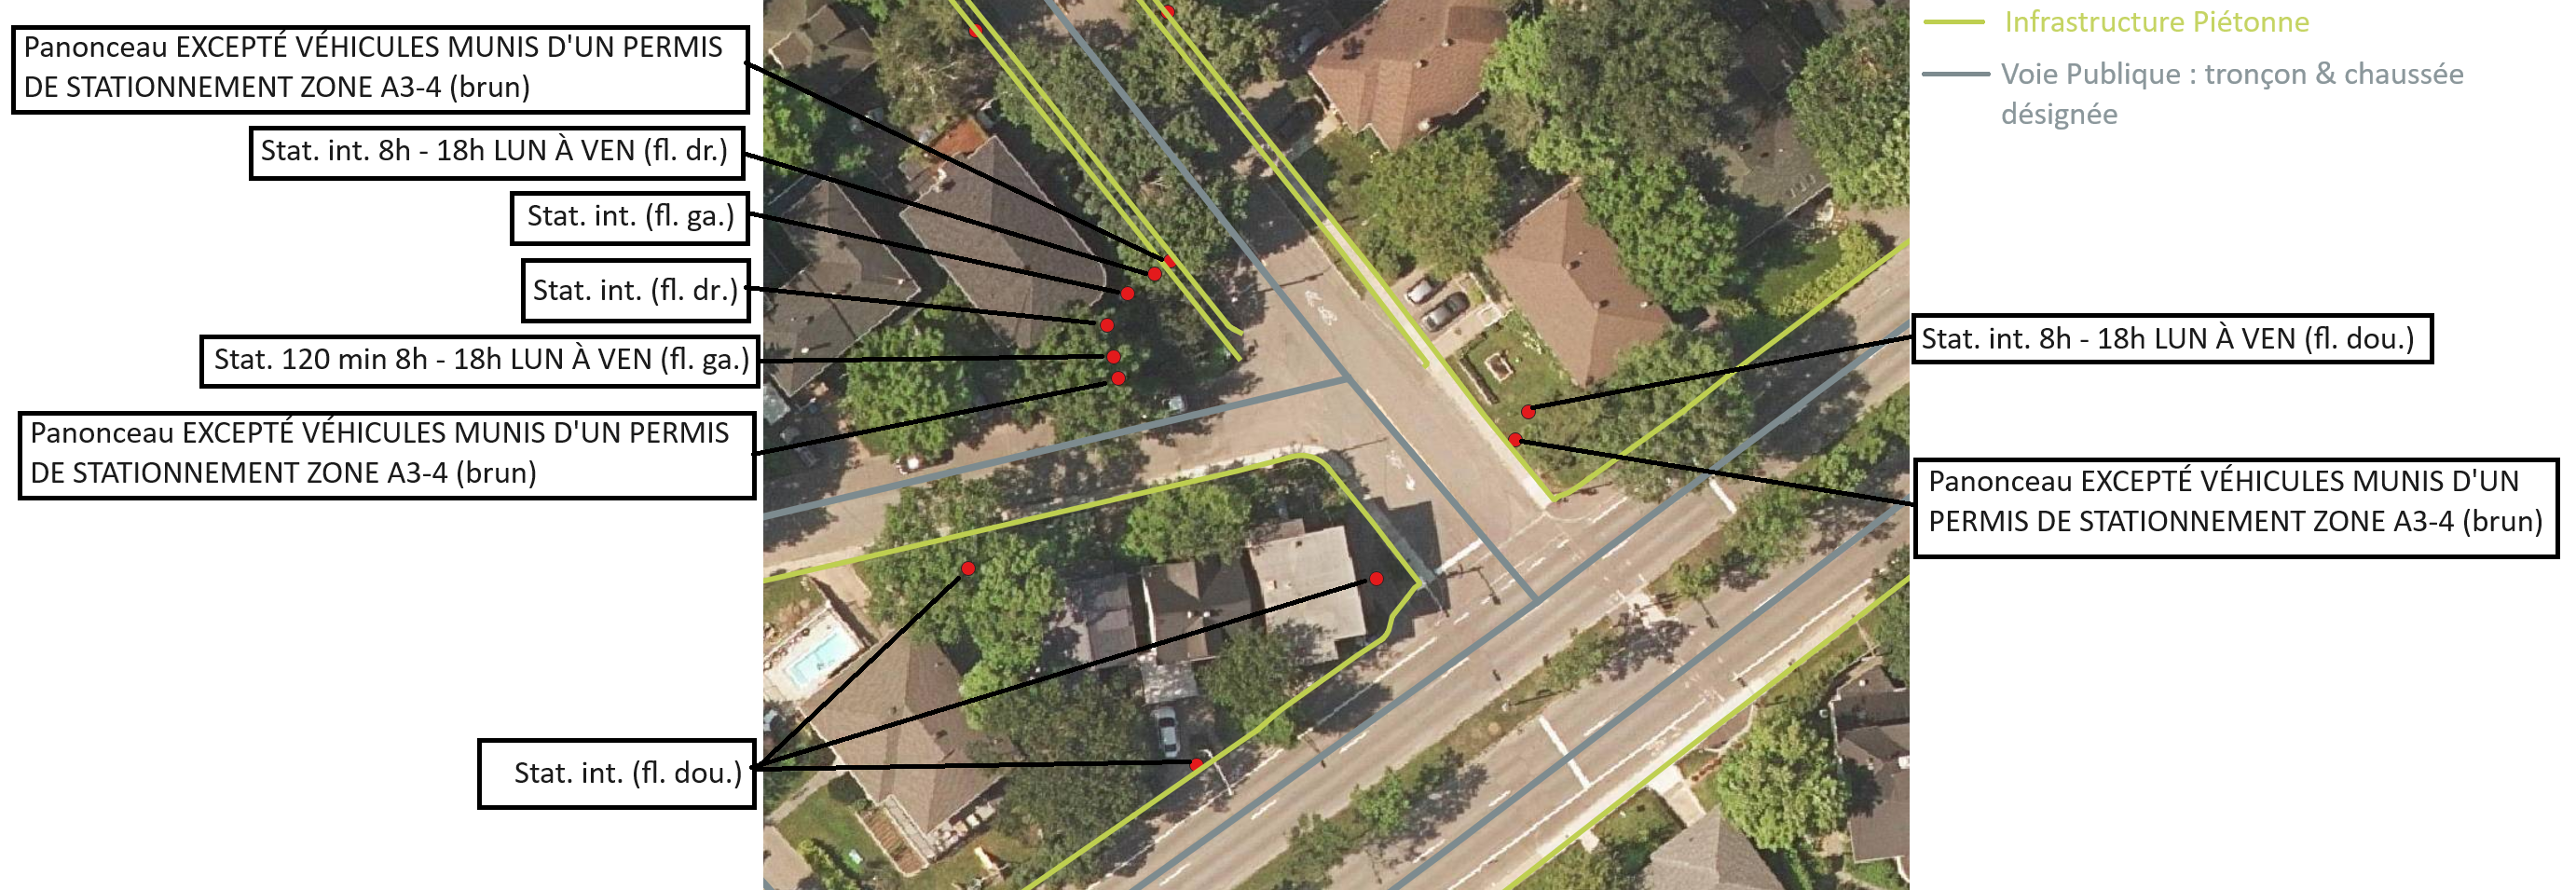
\includegraphics[width=1.0\textwidth]{images/enjeux_BD_panneaux_stationnement_Laurier.png}
    \caption{Exemple de panneaux sur un même poteau à endroits différents}
    \label{fig:enjeux_panneaux_Laurier}
  \end{figure}
  \begin{figure}[ht]
    \centering
    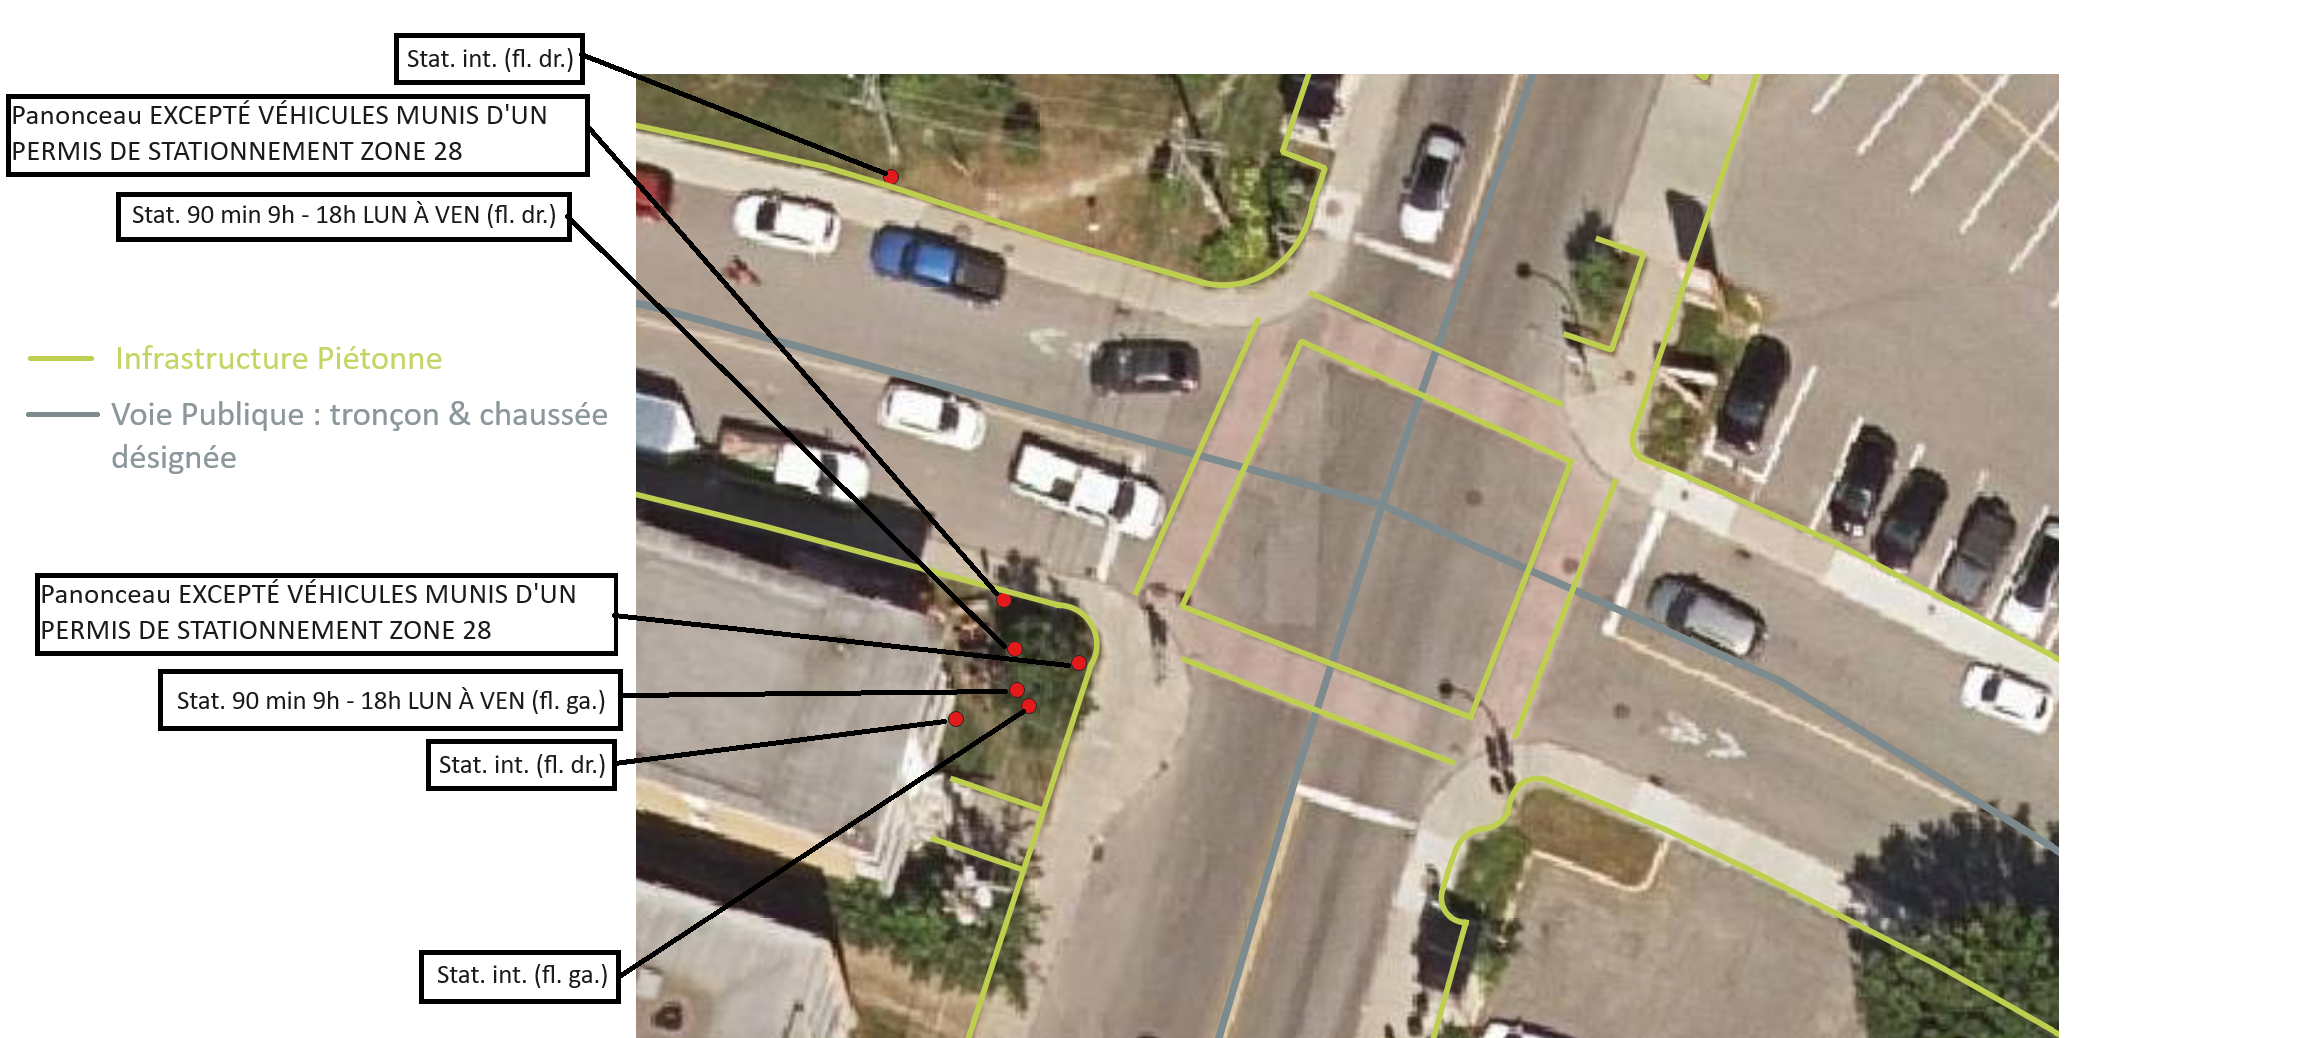
\includegraphics[width=1.0\textwidth]{images/enjeux_BD_panneaux_stationnement_Desroches.png}
    \caption{Exemple de panneaux sur un même poteau à endroits différents}
    \label{fig:enjeux_panneaux_Desroches}
  \end{figure}

  \FloatBarrier